\documentclass[10pt,letterpaper]{article}
\usepackage[margin=0.75in]{geometry}
\usepackage{amsmath}
\usepackage{amsfonts}
\usepackage{amssymb}
\usepackage{graphicx}
\usepackage{cancel}
\usepackage{listings}
\usepackage{color}
\usepackage{textcomp}
\definecolor{listinggray}{gray}{0.9}
\definecolor{lbcolor}{rgb}{0.9,0.9,0.9}
\lstset{
	backgroundcolor=\color{lbcolor},
	tabsize=4,
	rulecolor=,
% 	language=Python,
        basicstyle=\scriptsize,
        upquote=true,
        aboveskip={1.5\baselineskip},
        columns=fixed,
        showstringspaces=false,
        extendedchars=true,
        breaklines=true,
        prebreak = \raisebox{0ex}[0ex][0ex]{\ensuremath{\hookleftarrow}},
        frame=single,
        showtabs=false,
        showspaces=false,
        showstringspaces=false,
        identifierstyle=\ttfamily,
        keywordstyle=\color[rgb]{0,0,1},
        commentstyle=\color[rgb]{0.133,0.545,0.133},
        stringstyle=\color[rgb]{0.627,0.126,0.941},
}

\def\mbf{\mathbf}
\def\mbb{\mathbb}

\providecommand{\abs}[1]{\left\lvert#1\right\rvert}
\providecommand{\norm}[1]{\left\lVert#1\right\rVert}
\def\d{\mathrm{d}}
\def\e{\mathrm{e}}

\def\y{\mathbf{y}}
\def\f{\mathbf{f}}
\def\g{\mathbf{g}}
\def\b{\mathbf{b}}

\title{Numerical Treatment of Differential Equations: HW 1}
\author{Truman Ellis}

\begin{document}
\maketitle

\section*{Problem 1.1}
Apply the method of proof of Theorems 1.1 and 1.2 to prove the convergence of the implicit midpoint rule and of the theta method.

\subsection*{Solution}
\paragraph*{Implicit Midpoint Rule} We first need to calculate the local truncation error from
\begin{equation}\label{eq:LTE1}
y(t_{n+1})-y(t_n)-hf\left(t_n+\frac{h}{2},y\left(t_n+\frac{h}{2}\right)\right)\,.
\end{equation}
Substituting $f(t_n+\frac{h}{2},y(t_n+\frac{h}{2})) = y'(t_n+\frac{h}{2})$, and Taylor expanding
\[
y'\left(t_n+\frac{h}{2}\right)=y'(t_n)+\frac{h}{2}h''(t_n)+O(h^2)\,.
\]
Now, Taylor expanding 
\[
y(t_{n+1})=y(t_n)+hy'(t_n)+\frac{1}{2}h^2y''(t_n)+O(h^3)\,.
\]
We can substitute these into Equation \ref{eq:LTE1}:
\begin{align*}
&\cancel{y(t_n)}+h\cancel{y'(t_n)}+\frac{1}{2}h^2\cancel{y''(t_n)}+O(h^3)\\
&-\cancel{y(t_n)}\\
&-h(\cancel{y'(t_n)}+\frac{h}{2}h\cancel{y''(t_n)}+O(h^2))
&=O(h^3)\,.
\end{align*}
Now we can calculate the global error. Let us first Taylor expand $y(t_{n+1})$:
\begin{align*}
y(t_{n+1})&=y(t_n)+hy'(t_n)+\frac{h^2}{2}y''(t_n)+\frac{h^3}{6}y'''(t_n)+\cdots\\
&=y(t_n)+h[\underbrace{y'(t_n)+\frac{h}{2}y''(t_n)+\frac{h^2}{6}y'''(t_n)+\cdots}_
{\displaystyle y'\left(t_n+\frac{h}{2}\right)}
]\\
&=y(t_n)+h\left[y'\left(t_n+\frac{h}{2}\right)\right]\,.
\end{align*}
Now we can subtract
\begin{align*}
e_{n+1}&=y_{n+1}-y(t_{n+1})\\
&=y_n-y(t_n)+h\left[f\left(t_{n+\frac{1}{2}},\frac{1}{2}(y_n+y_{n+1})\right)\right]-h\left[y'\left(t_n+\frac{h}{2}\right)\right]+O(h^3)\\
&=e_n+h\left[f\left(t_n+\frac{h}{2},\frac{1}{2}(y_n+y_{n+1})\right)-f\left(t_n+\frac{h}{2},y(t_n+\frac{h}{2})\right)\right]+O(h^3)\,.
\end{align*}
Since $f$ is Lipshitz,
\begin{align*}
\norm{e_{n+1}}&\leq\norm{e_n}+h\norm{f\left(t_n+\frac{h}{2},\frac{1}{2}(y_n+y_{n+1})\right)-f\left(t_n+\frac{h}{2},y(t_n+\frac{h}{2})\right)}+Ch^3\\
&\leq\norm{e_n}+h\lambda\norm{\frac{1}{2}(y_n+y_{n+1})-y\left(t_n+\frac{h}{2}\right)}+Ch^3\\
&\leq\norm{e_n}+h\lambda\norm{\frac{1}{2}(y_n+y_{n+1})-\frac{1}{2}\left(y(t_n)+y(t_{n+1})\right)}+Ch^3\\
&\leq(1+\frac{1}{2}\lambda h)\norm{e_n}+\frac{1}{2}\lambda h\norm{e_{n+1}}+Ch^3\\
&\leq\frac{1+\frac{1}{2}\lambda h}{1-\frac{1}{2}\lambda h}\norm{e_n}+\frac{C}{1-\frac{1}{2}\lambda h}h^3
\end{align*}
We can now claim that 
\[
\norm{e_n}\leq\frac{C}{\lambda}\left[\left(\frac{1+\frac{1}{2}h\lambda}{1-\frac{1}{2}h\lambda}\right)^n-1\right]h^2\,.
\]
Indeed for $n=0$, $\norm{e_n}=0$ and 
\begin{align*}
\norm{e_{n+1}}&\leq\left(\frac{1+\frac{1}{2}h\lambda}{1-\frac{1}{2}h\lambda}\right)\norm{e_n}+\frac{C}{1-\frac{1}{2}\lambda h}h^3\\
&=\frac{C}{\lambda}h^2\left(\frac{1+\frac{1}{2}h\lambda}{1-\frac{1}{2}h\lambda}\right)^{n+1}
-\frac{C}{\lambda}\left(\frac{1+\frac{1}{2}h\lambda}{1-\frac{1}{2}h\lambda}\right)h^2+\frac{C}{\lambda}\frac{h^3\lambda}{1-\frac{1}{2}h\lambda}\\
&=\frac{C}{\lambda}h^2\left(\frac{1+\frac{1}{2}h\lambda}{1-\frac{1}{2}h\lambda}\right)^{n+1}
+\frac{C}{\lambda}\left(-\frac{h^2-\frac{1}{2}h^3\lambda+h^3\lambda}{1-\frac{1}{2}h\lambda}\right)\\
&=\frac{C}{\lambda}h^2\left(\frac{1+\frac{1}{2}h\lambda}{1-\frac{1}{2}h\lambda}\right)^{n+1}
+\frac{C}{\lambda}h^2\\
&=\frac{C}{\lambda}\left[\left(\frac{1+\frac{1}{2}h\lambda}{1-\frac{1}{2}h\lambda}\right)^{n+1}-1\right]h^2\,.
\end{align*}
Therefore the proof holds by induction, the implicit midpoint rule is order 2.

\paragraph*{Theta Method} We first need to calculate the local truncation error:
\begin{align*}
&y(t_{n+1})-\left[y(t_n)+h(\theta f(t_n,y(t_n))+(1-\theta)f(t_{n+1},y(t_{n+1})))\right]\\
&=\left[\cancel{y(t_n)}+h\cancel{y'(t_n)}+\frac{1}{2}h^2y''(t_n)+O(h^3)\right]\\
&-\left[\cancel{y(t_n)}+h\theta\cancel{y'(t_n)}+(1-\theta)h(\cancel{y'(t_n)}+hy''(t_n)+\frac{h^2}{2}y'''(t_n)+O(h^3))\right]\\
&=\left(\theta-\frac{1}{2}\right)h^2y''(tn)+\left(\frac{\theta}{2}-\frac{1}{3}\right)h^3y'''(t_n)+O(h^4)\,.
\end{align*}
Therefore the local truncation is order $h^2$ for $\theta=\frac{1}{2}$ and order $h$ otherwise.

Now for $\theta=\frac{1}{2}$, subtracting
\begin{align*}
e_{n+1}&=y_{n+1}-y(t_{n+1})\\
&=y_n+\frac{h}{2}(f(t_n,y_n)+f(t_{n+1},y_{n+1}))\\
&-y(t_n)-\frac{h}{2}(f(t_n,y(t_n))+f(t_{n+1},y(t_{n+1})))+O(h^3)\\
&=e_n+\frac{h}{2}[f(t_n,y_n)-f(t_n,y(t_n))]\\
&+\frac{h}{2}[f(t_{n+1},y_{n+1})-f(t_{n+1},y(t_{n+1}))]+O(h^3)\,.
\end{align*}
Since f is Lipshitz
\begin{align*}
\norm{e_{n+1}}&\leq\norm{e_n}+\frac{1}{2}\lambda h[\norm{y_n-y(t_n)}+\norm{y_{n+1}-y(t_{n+1})}]+Ch^3\\
&\leq\frac{1+\frac{1}{2}\lambda h}{1-\frac{1}{2}\lambda h}\norm{e_n}+\frac{C}{1-\theta\lambda h}h^3\\
&\leq\frac{C}{\lambda}\left[\left(\frac{1+\frac{1}{2}h\lambda}{1-\frac{1}{2}h\lambda}\right)^n-1\right]h^2\,.
\end{align*}
This indeed holds for $n=0$ and by induction for $n+1$:
\begin{align*}
\norm{e_{n+1}}&\leq\left(\frac{1+\frac{1}{2}h\lambda}{1-\frac{1}{2}h\lambda}\right)
\frac{C}{\lambda}h^2\left[\left(\frac{1+\frac{1}{2}h\lambda}{1-\frac{1}{2}h\lambda}\right)^n-1\right]
+\left(\frac{C}{1-\frac{1}{2}h\lambda}\right)h^3\\
&=\frac{C}{\lambda}\left[\left(\frac{1+\frac{1}{2}h\lambda}{1-\frac{1}{2}h\lambda}\right)^{n+1}-1\right]h^2\,.
\end{align*}
Therefore the theta method is order $h^2$ for $\theta=\frac{1}{2}$.

Now for $\theta\neq\frac{1}{2}$:
\begin{align*}
e_{n+1}&=y_{n+1}-y(t_{n+1})\\
&=y_n+h\theta f(t_n,y_n)+h(1-\theta)f(t_{n+1},y_{n+1})-y(t_n)-hf(t_n,y(t_n))+O(h^2)\\
&=y_n+h\theta f(t_n,y_n)-h(1-\theta)[f(t_n,y_n)+O(h)]-y(t_n)-hf(t_n,y(t_n))+O(h^2)\\
&=e_n+h[f(t_n,y_n)-f(t_n,y(t_n))]+O(h^2)\,.
\end{align*}
Since f is Lipshitz
\begin{align*}
\norm{e_{n+1}}&\leq(1+h\lambda)\norm{e_n}+Ch^2\\
&\leq\frac{C}{\lambda}\left[\left(1+h\lambda\right)^n-1\right]h\,.
\end{align*}
This indeed holds for $n=0$ and by induction for $n+1$:
\begin{align*}
\norm{e_{n+1}}&\leq(1+h\lambda)\frac{C}{\lambda}h[(1+h\lambda)^n-1]+Ch^2=\frac{C}{\lambda}h[(1+h\lambda)^{n+1}-1]
\end{align*}
Therefore the theta method is order $h$ for $\theta\neq\frac{1}{2}$.

\section*{Problem 1.3}
We solve the scalar linear system
\[
y'=ay\,,\quad y(0)=1\,.
\]
\paragraph*{a)} Show that the `continuous output' method
\[
u(t)=\frac{1+\frac{1}{2}a(t-nh)}{1-\frac{1}{2}a(t-nh)}y_n\,,\quad nh\leq t\leq(n+1)h\,,\quad n=0,1,...,
\]
is consistent with the values of $y_n$ and $y_{n+1}$ which are obtained by the trapezoid rule.

\subsection*{Solution}
According to the trapezoid rule
\[
y_{n+1}=y_n+\frac{1}{2}h[ay_n+ay_{n+1}]\,.
\]
Rearranging,
\begin{align*}
\left(1-\frac{1}{2}ha\right)y_{n+1}&=\left(1+\frac{1}{2}ha\right)y_n\\
y_{n+1}&=\frac{1+\frac{1}{2}ha}{1-\frac{1}{2}ha}y_n\,.
\end{align*}
Evaluating
\[
u(nh)=\frac{1+\frac{1}{2}a(0)}{1-\frac{1}{2}a(0)}y_n=y_n\,,
\]
this is consistent with the trapezoid rule. Again, evaluating
\[
u((n+1)h)=\frac{1+\frac{1}{2}a(h)}{1-\frac{1}{2}a(h)}y_n\,,
\]
this is also consistent with the results from the trapezoid rule.

\paragraph*{b)} Demonstrate that u obeys the perturbed ODE
\[
u'(t)=au(t)+\frac{\frac{1}{4}a^3(t-nh)^2}{\left[1-\frac{1}{2}a(t-nh)\right]^2}y_n\,\quad t\in[nh,(n+1)h]
\]
with initial condition $u(nh)=y_n$. Thus, prove that
\[
u((n+1)h)=\e^{ha}\left[1+\frac{1}{4}a^3\int_0^h\frac{\e^{-a\tau}\tau^2 d\tau\,\d\tau}{\left(1-\frac{1}{2}a\tau\right)^2}\right]y_n\,.
\]

\subsection*{Solution}
First we need to calculate
\begin{align*}
u'(t)&=-\frac{1+\frac{1}{2}a(t-nh)}{\left(1-\frac{1}{2}a(t-nh)\right)^2}\left(-\frac{1}{2}a\right)+\frac{\frac{1}{2}a}{1-\frac{1}{2}a(t-nh)}\\
&=\frac{a}{\left(1-\frac{1}{2}a(t-nh)\right)^2}y_n\,.
\end{align*}
Now, combining terms in the right hand side,
\begin{align*}
u'(t)&=a\left[\frac{1+\frac{1}{2}a(t-nh)}{1-\frac{1}{2}a(t-nh)}y_n\right]
+\frac{\frac{1}{4}a^3(t-nh)^2}{\left[1-\frac{1}{2}a(t-nh)\right]^2}y_n\,\quad t\in[nh,(n+1)h]\\
&=\frac{\left(a-\cancel{\frac{1}{4}a^3(t-nh)^2}\right)+\cancel{\frac{1}{4}a^3(t-nh)^2}}{\left(1-\frac{1}{2}a(t-nh)\right)^2}y_n\\
&=\frac{a}{\left(1-\frac{1}{2}a(t-nh)\right)^2}y_n\,.
\end{align*}
Therefore $u(t)$ does satisfy the perturbed ODE.

We now wish to find a solution via integrating factors. Let us rewrite
\[
u'(t)\underbrace{-a}_{\displaystyle P(t)}u(t)=\underbrace{\frac{\frac{1}{4}a^3(t-nh)^2}{\left[1-\frac{1}{2}a(t-nh)\right]^2}y_n}_{\displaystyle Q(t)}\,.
\]
Then,
\[
M(t)=\e^{\int P(t)\,\d t}=\e^{-at}\,.
\]
Now multiply both sides by $M(t)$, and using the product rule:
\begin{align*}
\e^{-at}u'(t)-a\e^{-at}u(t)&=\e^{-at}Q(t)\\
\frac{\d}{\d t}\left(\e^{-at}u(t)\right)=\e^{-at}Q(t)\,.
\end{align*}
Now integrate both sides from $nh$ to $(n+1)h$:
\[
\e^{-a(n+1)h}u((n+1)h)-\e^{-anh}u(nh)=\int_{nh}^{(n+1)h}\e^{-at}\frac{\frac{1}{4}a^3(t-nh)^2}{\left[1-\frac{1}{2}a(t-nh)\right]^2}y_n\,\d t\,.
\]
Simplifying,
\[
u((n+1)h)=\frac{1}{4}a^3\e^{a(n+1)h}\int_{nh}^{(n+1)h}\frac{\e^{-at}(t-nh)^2}{\left[1-\frac{1}{2}a(t-nh)\right]^2}y_n\,\d t
+\e^{ah}\underbrace{u(nh)}_{\displaystyle y_n}\,.
\]
Performing a change of variables to $\tau=t-nh$,
\begin{align*}
u((n+1h)&=\frac{1}{4}a^3\e^{a(n+1)h}\int_0^h\frac{\e^{-anh}\e^{-a\tau}\tau^2}{\left[1-\frac{1}{2}a\tau\right]^2}y_n\,\d\tau+\e^{ah}y_n\\
&=\frac{1}{4}a^3\e^{ah}\int_0^h\frac{\e^{-a\tau}\tau^2}{\left[1-\frac{1}{2}a\tau\right]^2}y_n\,\d\tau+\e^{ah}y_n\\
&=\e^{ah}\left[1+\frac{1}{4}a^3\int_0^h\frac{\e^{-a\tau}\tau^2}{\left[1-\frac{1}{2}a\tau\right]^2}y_n\,\d\tau\right]y_n\,.
\end{align*}

\paragraph*{c)} Let $e_n=y_n-y(nh)\,,\quad n=0,1,...,$ Show that 
\[
e_{n+1}=\e^{ha}\left[1+\frac{1}{4}a^3\int_0^h\frac{\e^{-a\tau}\tau^2\,\d\tau}{(1-\frac{1}{2}a\tau)^2}\right]e_n
+\frac{1}{4}a^3\e^{(n+1)ha}\int_0^h\frac{\e^{-a\tau}\tau^2\,\d\tau}{(1-\frac{1}{2}a\tau)^2}\,.
\]
In particular, deduce that $a<0$ implies that the error propagates subject to the inequality
\[
\abs{e_{n+1}}\leq \e^{ah}\left(1+\frac{1}{4}\abs{a}^3\int_0^h\e^{-a\tau}\tau^2\,\d\tau\right)\abs{e_n}
+\frac{1}{4}\abs{a}^3\e^{(n+1)ha}\int_0^h\e^{-a\tau}\tau^2\,\d\tau\,.
\]

\subsection*{Solution}
We can trivially solve the original ODE for the exact solution:
\[
y(t)=\e^{at}\,.
\]
Then,
\begin{align*}
e_{n+1}&=y_{n+1}-y((n+1)h)=u((n+1)h)-\e^{a(n+1)h}\\
&=\e^{ah}\left(\frac{1}{4}a^3\int_0^h\frac{\e^{-a\tau}\tau^2\,\d\tau}{(1-\frac{1}{2}a\tau)^2}\underbrace{y_n}_{\displaystyle=e_n+y(nh)}
+\underbrace{y_n-\underbrace{\e^{anh}}_{\displaystyle=y(nh)}}_{\displaystyle=e_n}\right)\\
&=\e^{ha}\left(\frac{1}{4}a^3\int_0^h\frac{\e^{-a\tau}\tau^2\,\d\tau}{(1-\frac{1}{2}a\tau)^2}+1\right)e_n
+\frac{1}{4}a^3\e^{(n+1)ha}\int_0^h\frac{\e^{-a\tau}\tau^2\,\d\tau}{(1-\frac{1}{2}a\tau)^2}\,.
\end{align*}
In particular, when $a<0$, the denominator of the integrals, $(1-\frac{1}{2}a\tau)^2 > 1$ and we can bound the error by 
letting the denominator be unity (thereby increasing the overall integral value). By replacing the integral denominators in the previous equation, 
we thus bound the error:
\[
\abs{e_{n+1}}\leq \e^{ah}\left(1+\frac{1}{4}\abs{a}^3\int_0^h\e^{-a\tau}\tau^2\,\d\tau\right)\abs{e_n}
+\frac{1}{4}\abs{a}^3\e^{(n+1)ha}\int_0^h\e^{-a\tau}\tau^2\,\d\tau\,.
\]
\section*{Problem 1.5}
Provided that $\mbf{f}$ is analytic, it is possible to obtain from $\mbf{y}'=\mbf{f}(t,\mbf{y})$ and expression for the second derivative of $\mbf{y}$, 
namely $\mbf{y}''=\mbf{g}(t,\mbf{y})$ where
\[
\mbf{g}(t,\mbf{y})=\frac{\partial\mbf{f}(t,\mbf{y})}{\partial t}+\frac{\partial\mbf{f}(t,\mbf{y})}{\partial\mbf{y}}\mbf{f}(t,\mbf{y})\,.
\]
Find the orders of the methods
\[
\y_{n+1}=\y_n+h\f(t_n,\y_n)+\frac{1}{2}h^2\mbf{g}(t_n,\y_n)
\]
and
\[
\y_{n+1}=\y_n+\frac{1}{2}h\left[\f(t_n,\y_n)+\f(t_{n+1},\y_{n+1})\right]
+\frac{1}{12}h^2\left[\mbf{g}(t_n,\y_n)-\mbf{g}(t_{n+1},y_{n+1})\right]\,.
\]
\subsection*{Solution}
\paragraph*{a)} First, Taylor expand the exact solution
\[
\y(t_{n+1})=\y(t_n)+h\y'(t_n)+\frac{h^2}{2}\y''(t_n)+\frac{h^3}{6}\y'''(\xi)\,.
\]
Now, substituting $\y''(t_n)$ for $\mbf{g}(t_n,\y(t_n)$, compute
\begin{align*}
\y_{n+1}-\y(t_{n+1})&=\cancel{\y(t_n)}+h\cancel{\y'(t_n)}+\frac{h^2}{2}\cancel{\y''(t_n)}\\
&-\left[\cancel{\y(t_n)}+h\cancel{\y'(t_n)}+\frac{h^2}{2}\cancel{\y''(t_n)}+\frac{h^3}{6}\y'''(\xi)\right]\\
&=O(h^3)\,.
\end{align*}
Therefore the local truncation error is order $h^2$.

The global error can be found from:
\begin{align*}
e_{n+1}&=\y_{n+1}-\y(t_{n+1})\\
&=\y_n+h\f(t_n,\y_n)+\frac{h^2}{2}\g(t_n,y_n)-\y(t_n)+h\y'(t_n)-\frac{h^2}{2}\y''(t_n)+O(h^3)\\
&=e_n+h[\f(t_n,y(t_n)+e_n)-\f(t_n,\y(t_n))]+\frac{h^2}{2}[\g(t_n,\y(t_n)+e_n)-\g(t_n,\y(t_n))]+O(h^3)\\
\end{align*}
From the triangle inequality and the Lipshitz condition and assuming $h<1$, for appropriate $\lambda$:
\begin{align*}
\norm{e_{n+1}}&\leq\norm{e_n}+h\norm{\f(t_n,y(t_n)+e_n)-\f(t_n,\y(t_n))}+\frac{h^2}{2}\norm{\g(t_n,\y(t_n)+e_n)-\g(t_n,\y(t_n))}+Ch^3\\
&\leq(1+\underbrace{h\lambda_f+\frac{h^2}{2}}_{\displaystyle \leq h\lambda}\lambda_g)\norm{e_n}+Ch^3\\
&\leq\frac{C}{\lambda}h^2[(1+h\lambda)^n-1]\,.
\end{align*}
This indeed holds for $n=0$ and by induction for $n+1$:
\begin{align*}
\norm{e_{n+1}}&\leq(1+h\lambda)\frac{C}{\lambda}h^2[(1+h\lambda)^n-1]+Ch^3=\frac{C}{\lambda}h^2[(1+h\lambda)^{n+1}-1]
\end{align*}
Therefore the method is order $h^2$.

\paragraph*{b)} First we need to compute a few Taylor expansions:
\begin{align*}
\y(t_{n+1})&=\y(t_n)+h\y'(t_n)+\frac{h^2}{2}\y''(t_n)+\frac{h^3}{6}\y'''(t_n)+\frac{h^4}{24}\y^{(4)}(t_n)+\frac{h^4}{120}\y^{(5)}(t_n)+O(h^6)\,,\\
\y'(t_{n+1})&=\y'(t_n)+h\y''(t_n)+\frac{h^2}{2}\y'''(t_n)+\frac{h^3}{6}\y^{4)}(t_n)+\frac{h^5}{24}\y^{(5)}(t_n)+O(h^5)\,,\\
\y''(t_{n+1})&=\y''(t_n)+h\y'''(t_n)+\frac{h^2}{2}\y^{(4)}(t_n)+\frac{h^3}{6}\y^{5)}(t_n)+O(h^4)\,.\\
\end{align*}
Now compute
\begin{align*}
\y_{n+1}-\y(t_{n+1})&=
\y_n+\frac{1}{2}h\left[\f(t_n,\y_n)+\f(t_{n+1},\y_{n+1})\right]
+\frac{1}{12}h^2\left[\mbf{g}(t_n,\y_n)-\mbf{g}(t_{n+1},\y_{n+1})\right]\\
&-\left(\y(t_n)+h\y'(t_n)+\frac{h^2}{2}\y''(t_n)+\frac{h^3}{6}\y'''(t_n)
+\frac{h^4}{24}\y^{(4)}(t_n)+\frac{h^4}{120}\y^{(5)}(t_n)+O(h^6)\right)\\
&=\y_n
+\frac{1}{2}h\left[\y'(t_n)+\y'(t_{n+1})\right]\\
&+\frac{1}{12}h^2\left[\y''(t_n)-\y''(t_{n+1})\right]\\
&-\left(\y(t_n)+h\y'(t_n)+\frac{h^2}{2}\y''(t_n)+\frac{h^3}{6}\y'''(t_n)
+\frac{h^4}{24}\y^{(4)}(t_n)+\frac{h^4}{120}\y^{(5)}(t_n)+O(h^6)\right)\\
&=\y_n
+\frac{1}{2}h\left[\y'(t_n)+\y'(t_n)+h\y''(t_n)+\frac{h^2}{2}\y'''(t_n)+\frac{h^3}{6}\y^{4)}(t_n)+\frac{h^5}{24}\y^{(5)}(t_n)+O(h^5)\right]\\
&+\frac{1}{12}h^2\left[\y''(t_n)-\y''(t_n)-h\y'''(t_n)-\frac{h^2}{2}\y^{(4)}(t_n)-\frac{h^3}{6}\y^{5)}(t_n)-O(h^4)\right]\\
&-\left(\y(t_n)+h\y'(t_n)+\frac{h^2}{2}\y''(t_n)+\frac{h^3}{6}\y'''(t_n)
+\frac{h^4}{24}\y^{(4)}(t_n)+\frac{h^4}{120}\y^{(5)}(t_n)+O(h^6)\right)\\
&=\left(1-1\right)\y(t_n)+\left(\frac{1}{2}+\frac{1}{2}-1\right)h\y'(t_n)
+\left(\frac{1}{2}+\frac{1}{12}-\frac{1}{12}-\frac{1}{12}\right)\frac{h^2}{2}\y''(t_n)\\
&+\left(\frac{1}{4}-\frac{1}{12}-\frac{1}{6}\right)\frac{h^3}{6}\y'''(t_n)
+\left(\frac{1}{12}-\frac{1}{24}-\frac{1}{24}\right)\frac{h^4}{24}\y^{(4)}(t_n)\\
&+\left(\frac{1}{48}-\frac{1}{72}-\frac{1}{120}\right)\frac{h^4}{120}\y^{(5)}(t_n)+O(h^6)\\
&=O(h^5)\,.
\end{align*}
Therefore the local truncation error is order $h^4$.

Subtracting 
\[
\y(t_{n+1})=\y(t_n)+\frac{h}{2}[\f(t_n,\y(t_n))+\f(t_{n+1},\y(t_{n+1}))]
+\frac{h^2}{12}[\g(t_n,\y(t_n))+\g(t_{n+1},\y(t_{n+1}))]+O(h^5)
\]
from $y_{n+1}$, we obtain
\begin{align*}
e_{n+1}&=e_n+\frac{h}{2}\left\{[\f(t_n,\y_n)-\f(t_n,\y(t_n))]+[\f(t_{n+1},\y_{n+1})-\f(t_{n+1},\y(t_{n+1}))]\right\}\\
&+\frac{h^2}{12}\left\{[\g(t_n,\y_n)-\g(t_n,\y(t_n))]+[\g(t_{n+1},\y_{n+1})-\g(t_{n+1},\y(t_{n+1}))]\right\}+O(h^5)\,.
\end{align*}
From Lipshitz and the triangle inequality,
\begin{align*}
\norm{e_{n+1}}&\leq\norm{e_n}+\frac{h}{2}\left\{\norm{\f(t_n,\y_n)-\f(t_n,\y(t_n))}+\norm{\f(t_{n+1},\y_{n+1})-\f(t_{n+1},\y(t_{n+1}))}\right\}\\
&+\frac{h^2}{12}\left\{\norm{\g(t_n,\y_n)-\g(t_n,\y(t_n))}+\norm{\g(t_{n+1},\y_{n+1})-\g(t_{n+1},\y(t_{n+1}))}\right\}+Ch^5\\
&\leq\frac{1+\frac{1}{2}h\lambda_f+\frac{1}{12}h^2\lambda_g}{1-\frac{1}{2}h\lambda_f-\frac{1}{12}h^2\lambda_g}\norm{e_n}
+\frac{C}{1-\frac{1}{2}h\lambda_f-\frac{1}{12}h^2\lambda_g}h^5\,.
\end{align*}
Assuming $h<1$, the inequality is still satisfied if we substitute $\frac{1}{2}h\lambda_f+\frac{1}{12}h^2\lambda_g$ with appropriate $\frac{1}{2}h\lambda$:
\begin{align*}
\norm{e_{n+1}}&\leq\frac{1+\frac{1}{2}h\lambda}{1-\frac{1}{2}h\lambda}\norm{e_n}+\frac{C}{1-\frac{1}{2}h\lambda}h^5\\
&\leq\frac{C}{\lambda}\left[\left(\frac{1+\frac{1}{2}h\lambda}{1-\frac{1}{2}h\lambda}\right)^n-1\right]h^4\,.
\end{align*}
This is indeed satisfied for $n=0$ and by induction for $n+1$:
\begin{align*}
\norm{e_{n+1}}&\leq\left(\frac{1+\frac{1}{2}h\lambda}{1-\frac{1}{2}h\lambda}\right)
\frac{C}{\lambda}h^4\left[\left(\frac{1+\frac{1}{2}h\lambda}{1-\frac{1}{2}h\lambda}\right)^n-1\right]
+\left(\frac{C}{1-\frac{1}{2}h\lambda}\right)h^5\\
&=\frac{C}{\lambda}\left[\left(\frac{1+\frac{1}{2}h\lambda}{1-\frac{1}{2}h\lambda}\right)^{n+1}-1\right]h^4\,.
\end{align*}
Therefore the method is order $h^4$.

\section*{Problem 1.7}
Repeated differentiation of the ODE, for analytic $\f$ yields explicit expressions for functions $\g_m$ such that
\[
\frac{\d^m\y(t)}{\d t^m}=\g_m(t,\y(t))\,,\quad m=0,1,...
\]
Hence $\g_0(t,\y)=\y$ and $\g_1(t,\y)=\f(t,\y)$.
\paragraph*{a)} Assuming for simplicity that $\f=\f(\y)$ (i.e. that the ODE system is autonomous), derive $\g_3$.
\subsection*{Solution}
\begin{align*}
\g_3(t,\y)&=\frac{\d^3\y(t)}{\d t^3}=\frac{\d}{\d t}\left(\frac{\d^2}{\d t^2}\right)
=\frac{\d}{\d t}\left(\frac{\d}{\d t}\left(\frac{\d y}{\d t}\right)\right)
=\frac{\d}{\d t}\left(\frac{\d}{\d t}(\f(\y))\right)
=\frac{\d}{\d t}\left(\frac{\d\f}{\d\y}\f\right)\\
&=\frac{\d^2\f}{\d y^2}\f^2+\left(\frac{\d\f}{\d y}\right)^2\f\,.
\end{align*}

\paragraph*{b)} Prove that the $m$th \emph{Taylor method}
\[
\y_{n+1}=\sum_{k=0}^n\frac{1}{k!}h^k\g_k(t_n,\y_n)\,,\quad n=0,1,...,
\]
is of order $m$ for $m=1,2,...$
\subsection*{Solution}
The exact Taylor expansion of $y(t_{n+1})$ can be written
\[
y(t_{n+1})=\sum_{k=0}^\infty\frac{1}{k!}h^k\g_k(t_n,\y_n)=\sum_{k=0}^m\frac{1}{k!}h^k\g_k(t_n,\y_n)+\frac{1}{(m+1)!}h^{m+1}\y^{(m+1)}(\xi)\,.
\]
Calculate:
\begin{align*}
y_{n+1}-y(t_{n+1})&=\sum_{k=0}^m\frac{1}{k!}h^k\g_k(t_n,\y_n)-\left(\sum_{k=0}^m\frac{1}{k!}h^k\g_k(t_n,\y_n)+\frac{1}{(m+1)!}h^{m+1}\y^{(m+1)}(\xi)\right)\\
&=-\frac{1}{(m+1)!}h^{m+1}\y^{(m+1)}(\xi)=O(h^{m+1})\,.
\end{align*}
Therefore the local truncation error is of order $h^m$.

The global error is
\begin{align*}
e_{n+1}&=\sum_{k=0}^m\frac{1}{k!}h^kg_k(t_n,y_n)-\sum_{k=0}^m\frac{1}{k!}h^kg_k(t_n,y(t_n))+O(h^{m+1})\\
&=\sum_{k=0}^m\frac{1}{k!}h^k(g_k(t_n,y_n)-g_k(t_n,y(t_n))+O(h^{m+1})\,.
\end{align*}
The Lipshitz condition gives us
\begin{align*}
\norm{e_{n+1}}&\leq\left(1+\sum_{k=1}^m\frac{1}{k!}h^k\lambda_k\right)\norm{e_n}+Ch^{m+1}\,.
\end{align*}
For $h<1$ and appropriate $\lambda$ we can say
\begin{align*}
\norm{e_{n+1}}&\leq\left(1+h\lambda\right)\norm{e_n}+Ch^{m+1}\\
&\leq\frac{C}{\lambda}h^m[(1+h\lambda)^n-1]\,.
\end{align*}
This indeed holds for $n=0$ and by induction for $n+1$:
\begin{align*}
\norm{e_{n+1}}&\leq(1+h\lambda)\frac{C}{\lambda}h^m[(1+h\lambda)^n-1]+Ch^{m+1}=\frac{C}{\lambda}h^m[(1+h\lambda)^{n+1}-1]
\end{align*}
Therefore the method is order $h^m$.

\paragraph*{c)} Let $\f(\y)=\Lambda\y+\b$, where the matrix $\Lambda$ and the vector $\b$ are independent of $t$. Find the explicit form of $\g_m$ for $m=0,1,\dots$ 
and thereby prove that the $m$th Taylor method reduces to the recurrence
\[
\y_{n+1}=\left(\sum_{k=0}^m\frac{1}{k!}h^k\Lambda^k\right)\y_n
+\left(\sum_{k=1}^m\frac{1}{k!}h^k\Lambda^{k-1}\right)\b\,,\quad n=0,1,\dots
\]
\subsection*{Solution}
Recall $\y'=\f(\y)$ and
\[
\g_m=\frac{\d^m\y}{\d t^m}\,.
\]
Then
\[
\g_2=\frac{\d}{\d t}(\f(\y))=\frac{\d}{\d t}(\Lambda\y+\b)=\Lambda\f=\Lambda^2\y+\Lambda\b\,,
\]
and
\[
\g_3=\frac{\d}{\d t}(\g_2)=\frac{\d}{\d t}(\Lambda^2\y+\Lambda\b)=\Lambda^2\f=\Lambda^3\y+\Lambda^2\b\,.
\]
A pattern becomes apparent, thus
\[
\g_m=\Lambda^m\y+\Lambda^{m-1}\b\,.
\]
We can substitute this into the formula for the $m$th order Taylor method and splitting the sum:
\begin{align*}
\y_{n+1}&=y_n+\sum_{k=1}^m\frac{1}{k!}h^k(\Lambda^m\y_n+\Lambda^{m-1}\b)\\
&=\left(\sum_{k=0}^m\frac{1}{k!}h^k\Lambda^k\right)y_n+\left(\sum_{k=1}^m\frac{1}{k!}h^k\Lambda^{k-1}\right)\b\,.
\end{align*}


\section*{Euler's Method}
\subsection*{Test Problem 1}
\begin{align*}
\f(t,\y) &= (-2y_1,-3y_2)\\
\y(0) &= (1, 2)
\end{align*}
Exact Solution:
\[
\y(t)=(y_1(0)\e^{-2t}, y_2(0)\e^{-3t})
\]
\begin{figure}[h!]
\centering
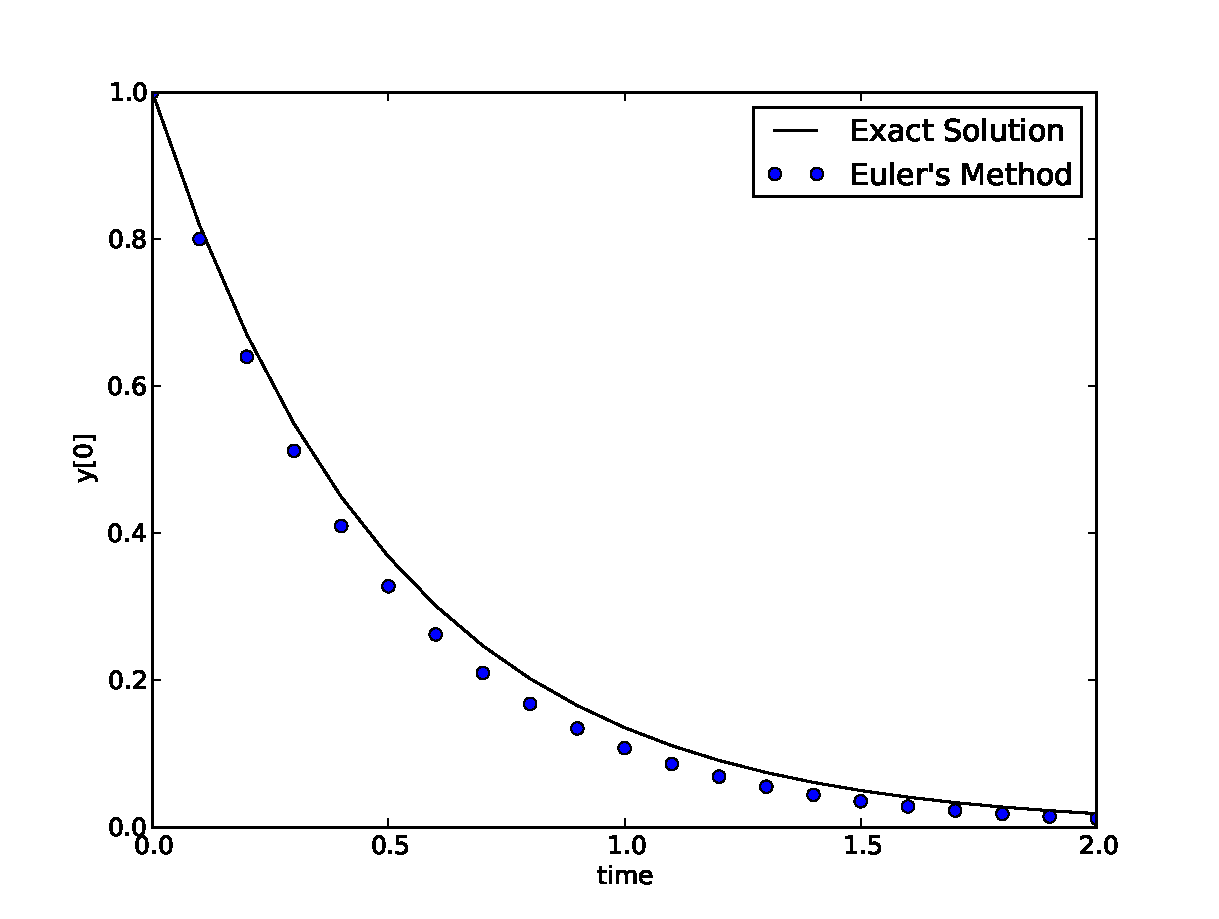
\includegraphics[width=3.25in,keepaspectratio=true]{./p1_1.pdf}
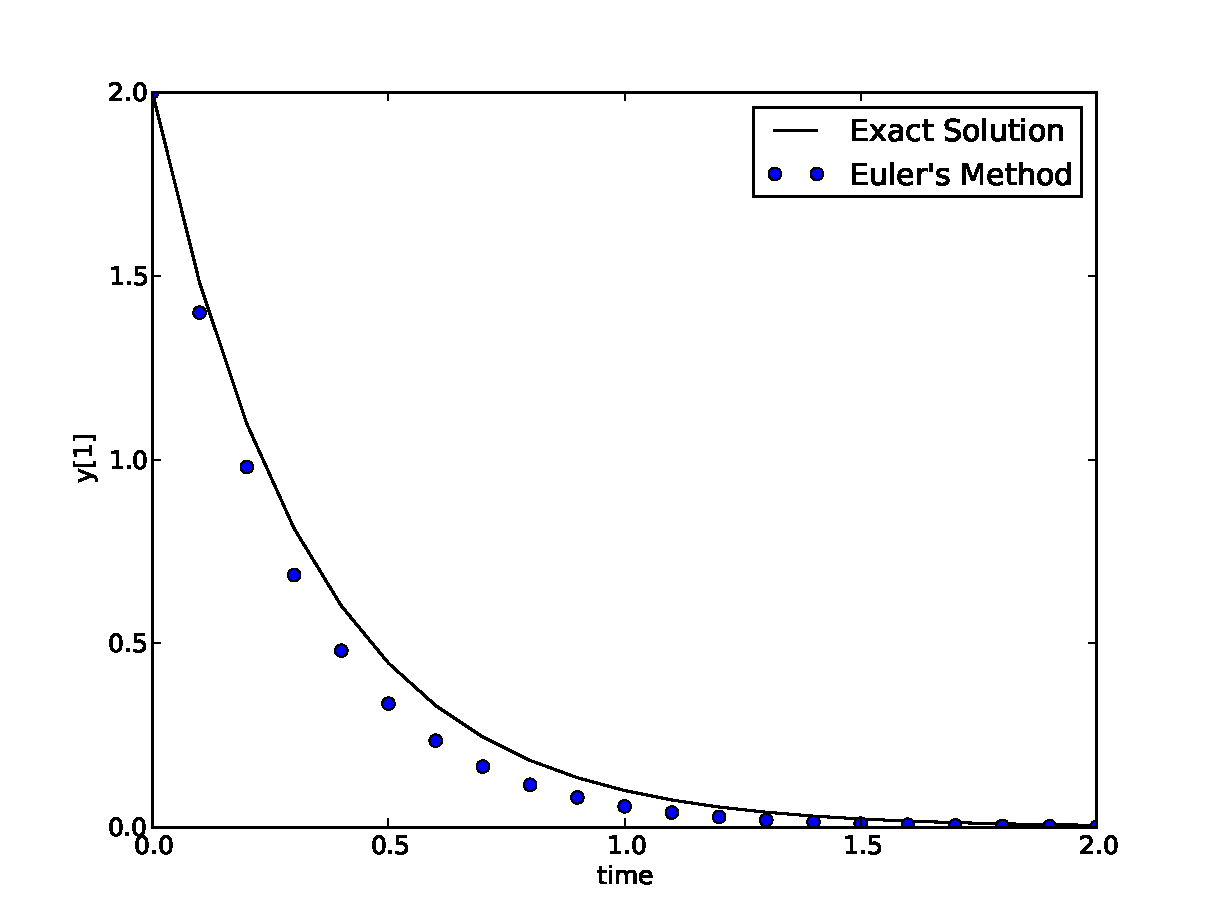
\includegraphics[width=3.25in,keepaspectratio=true]{./p1_2.pdf}
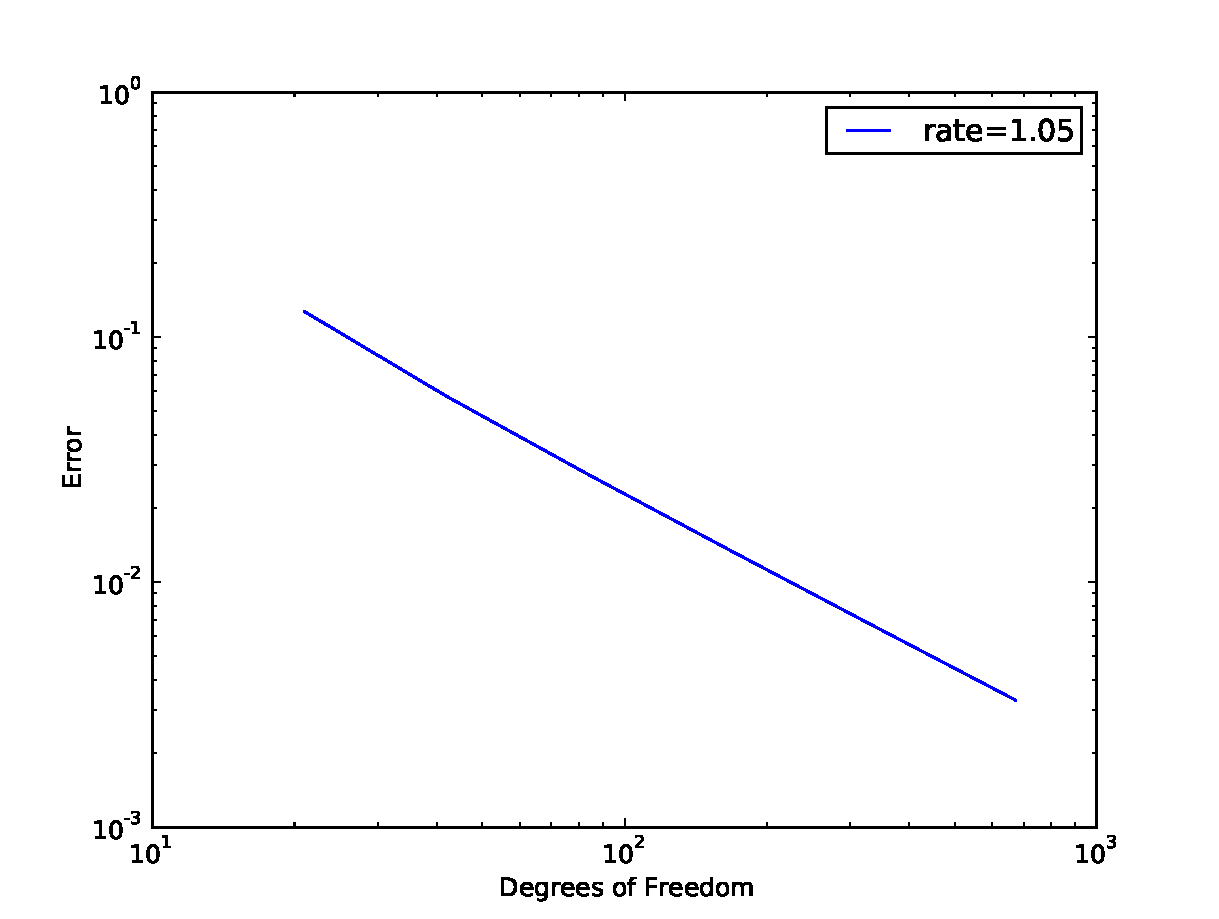
\includegraphics[width=4in,keepaspectratio=true]{./p1_3.pdf}
\caption{Problem 1}
\end{figure}

\subsection*{Test Problem 2}
\begin{align*}
\f(t,\y) &= (\frac{1}{2},-t)\\
\y(0) &= (3, 4)
\end{align*}
Exact Solution:
\[
\y(t)=(y_1(0)+0.5t, y_2(0)-0.5t^2)
\]
\begin{figure}[h!]
\centering
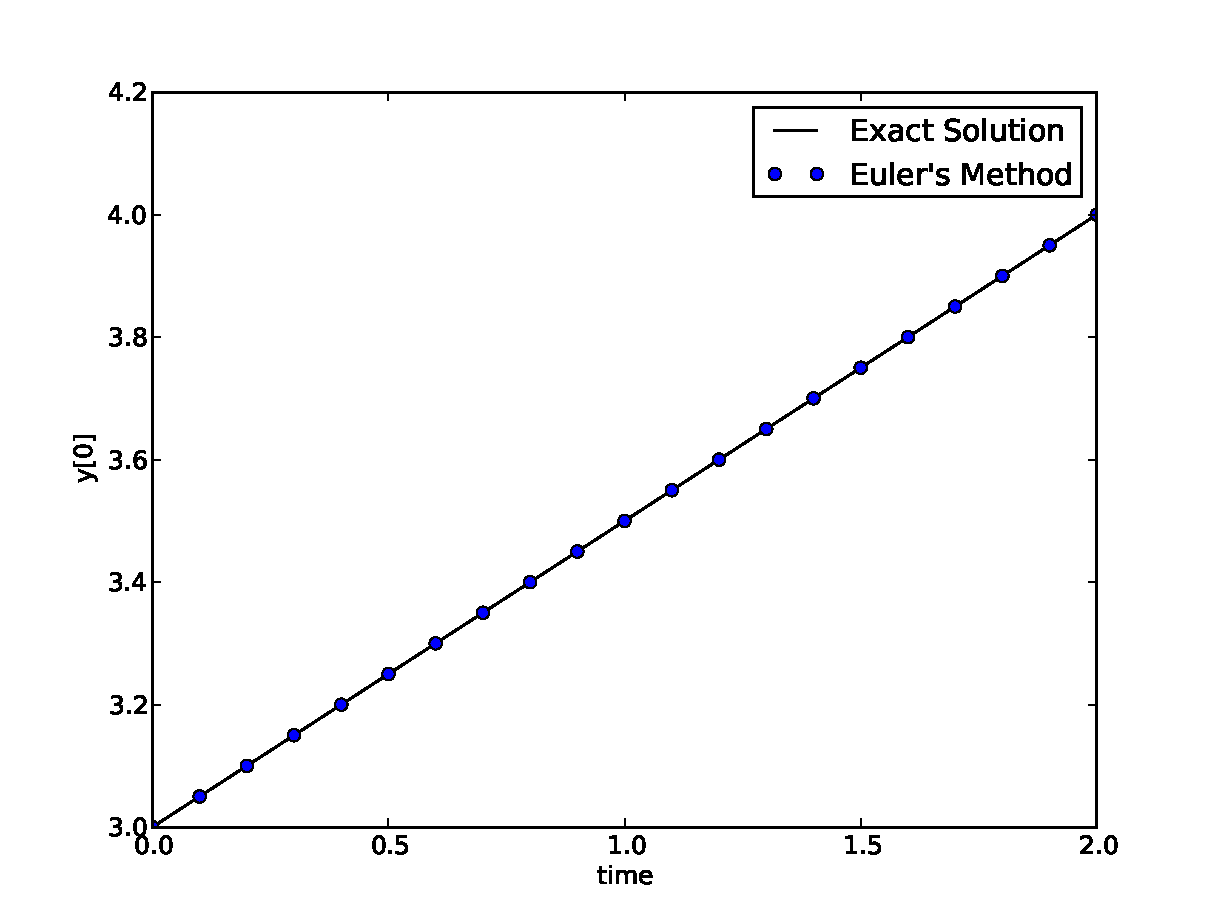
\includegraphics[width=3.25in,keepaspectratio=true]{./p2_1.pdf}
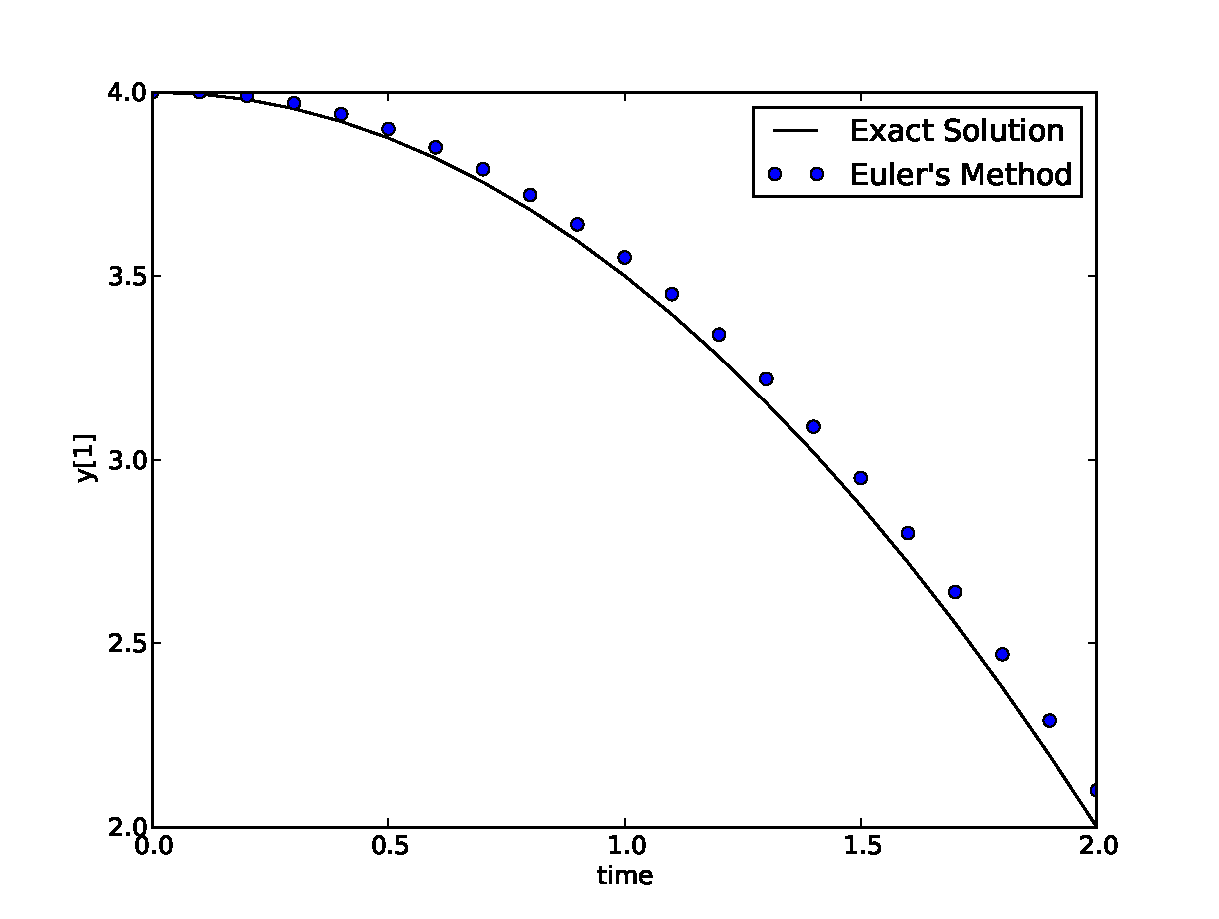
\includegraphics[width=3.25in,keepaspectratio=true]{./p2_2.pdf}
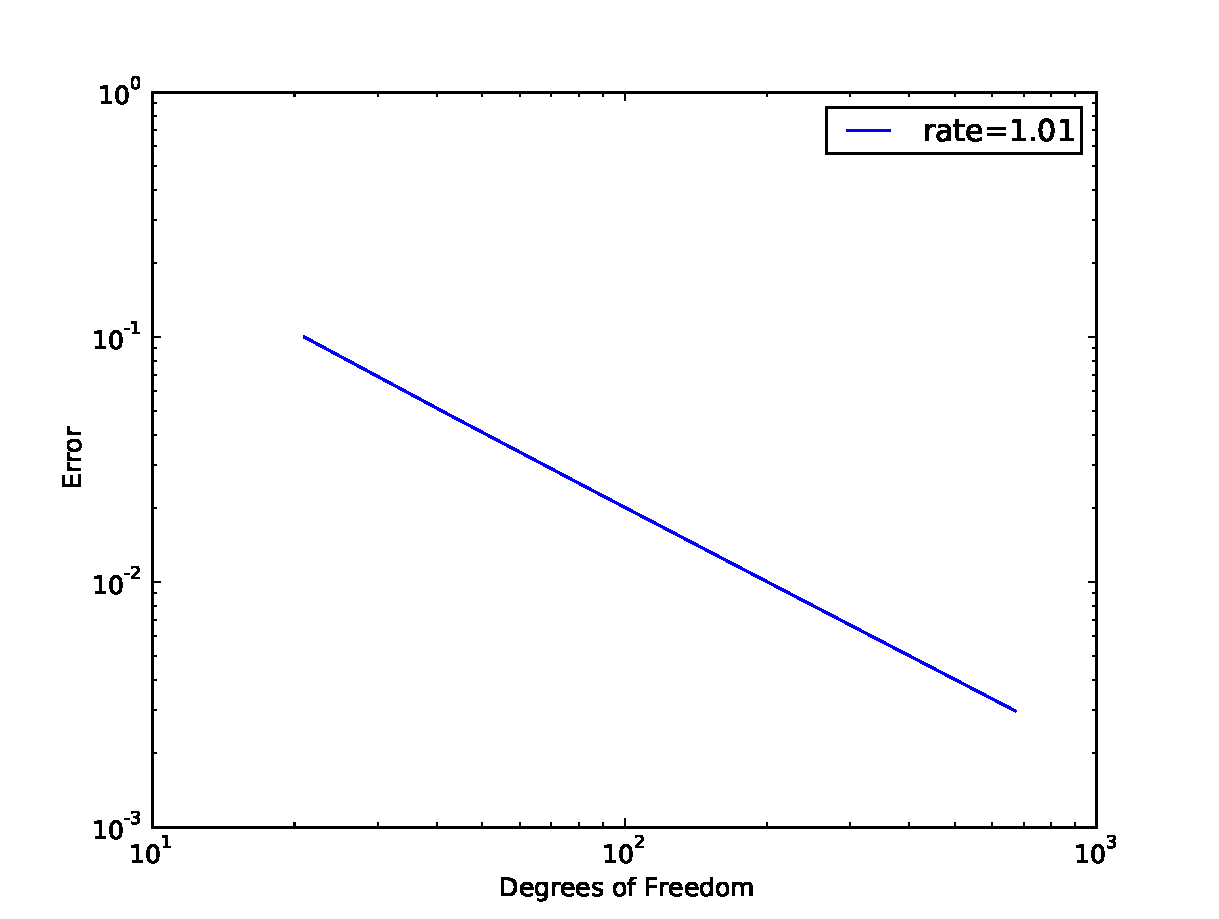
\includegraphics[width=4in,keepaspectratio=true]{./p2_3.pdf}
\caption{Problem 2}
\end{figure}

\subsection*{Test Problem 3}
\begin{align*}
\f(t,\y) &= -\y^2t\\
\y(0) &= 2
\end{align*}
Exact Solution:
\[
\y(t)=y(0)/(1+0.5t^2y(0))
\]
\begin{figure}[h!]
\centering
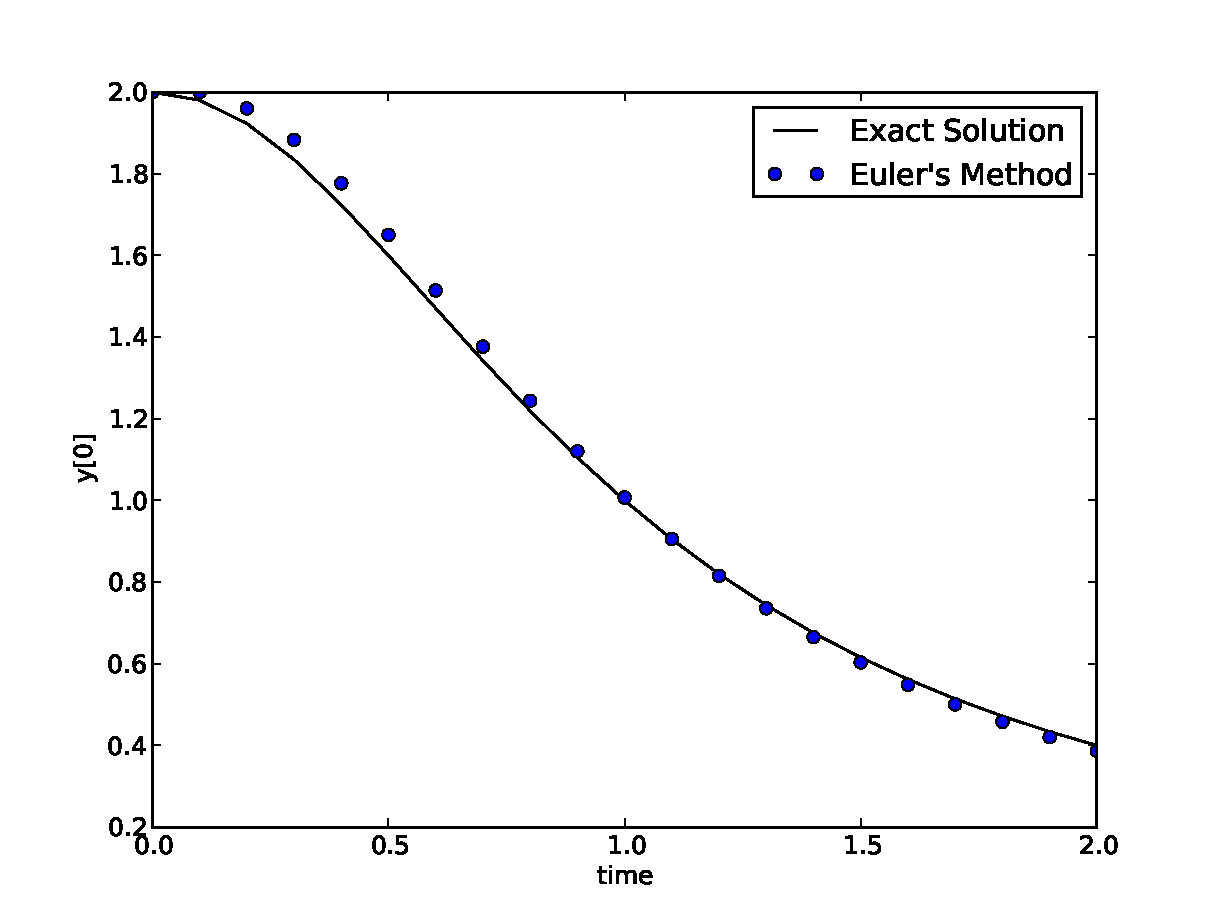
\includegraphics[width=3.25in,keepaspectratio=true]{./p3_1.pdf}
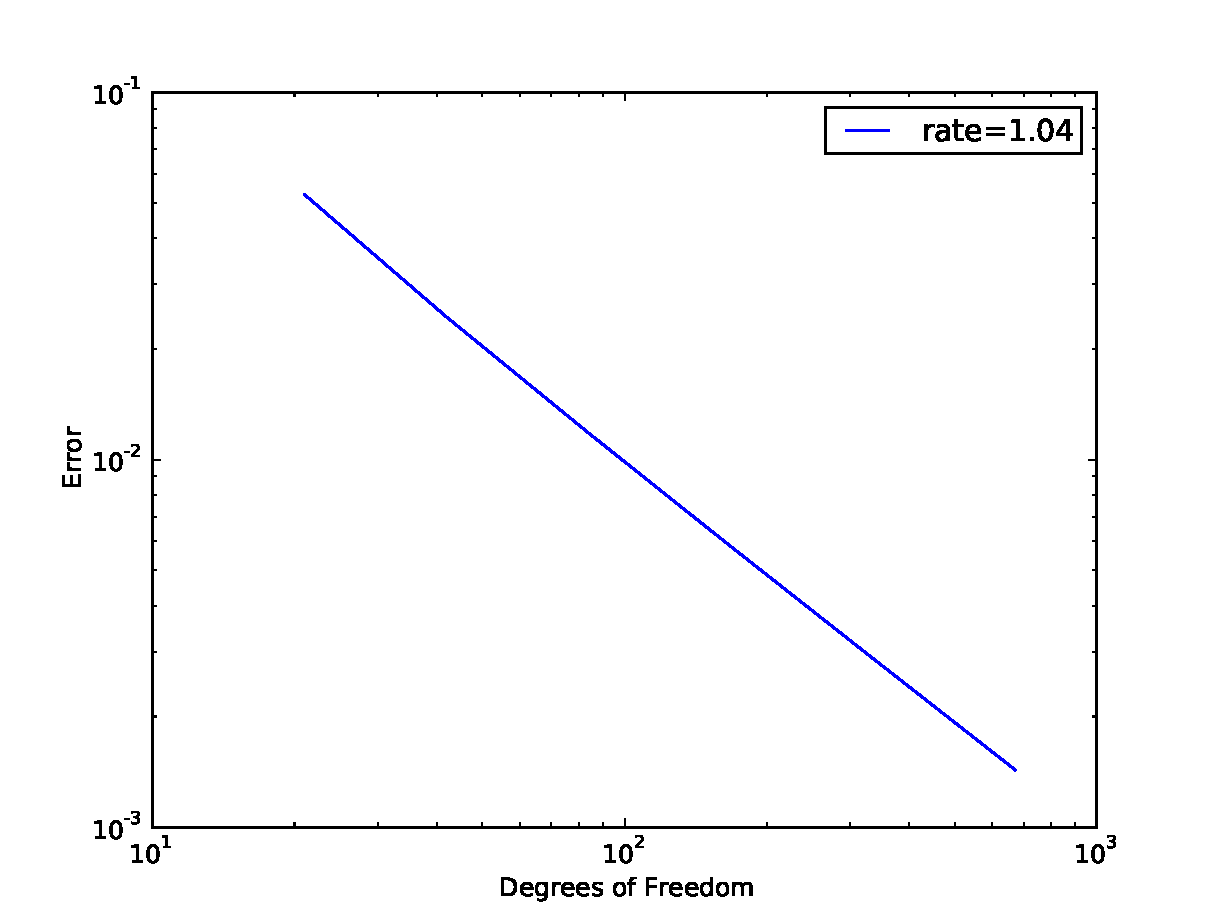
\includegraphics[width=3.25in,keepaspectratio=true]{./p3_2.pdf}
\caption{Problem 3}
\end{figure}

\subsection*{Test Problem 4}
\begin{align*}
\f(t,\y) &= (-y_1,y_1)\\
\y(0) &= (1, 2)
\end{align*}
Exact Solution:
\[
\y(t)=(y_1(0)\e^t, y_1(0)(1-\e^t)+y_2(0))
\]
\begin{figure}[h!]
\centering
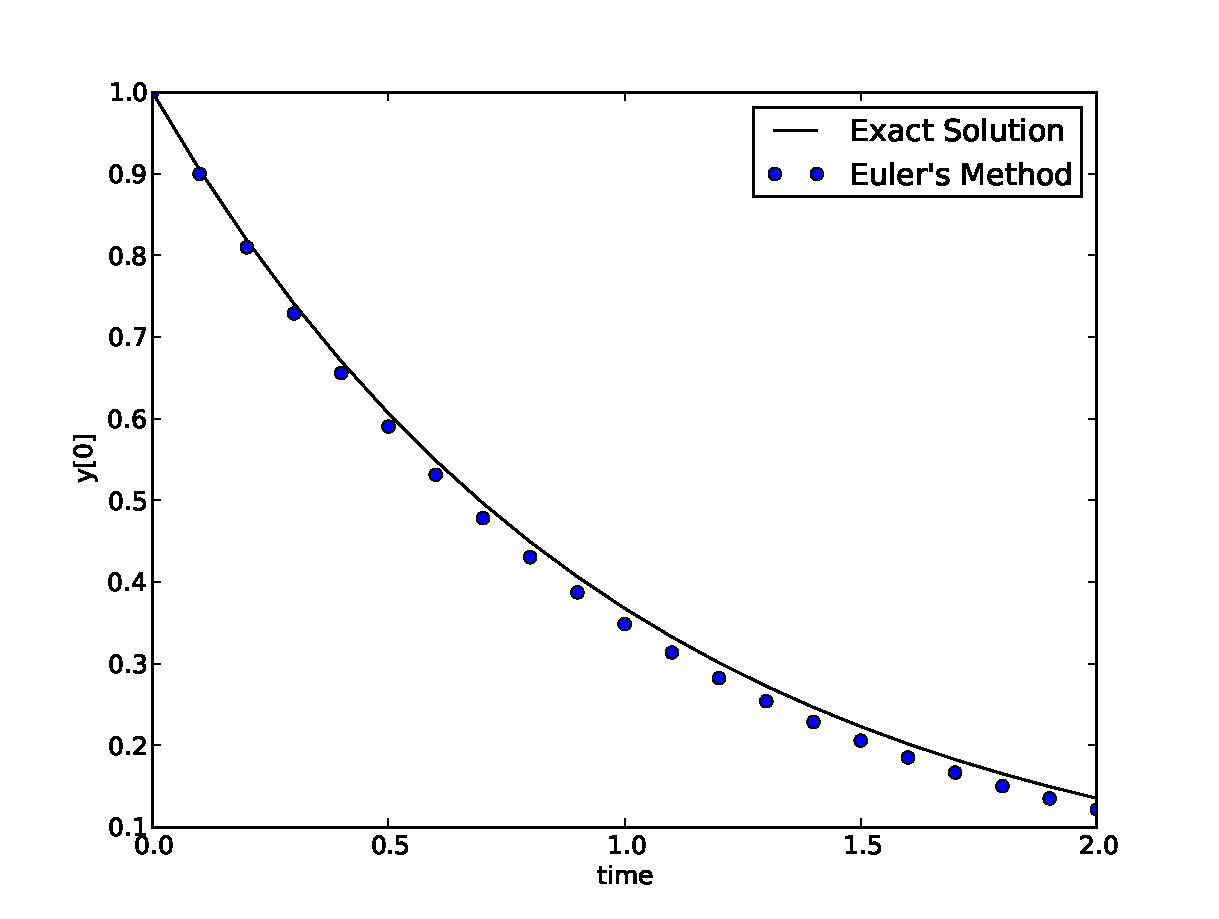
\includegraphics[width=3.25in,keepaspectratio=true]{./p4_1.pdf}
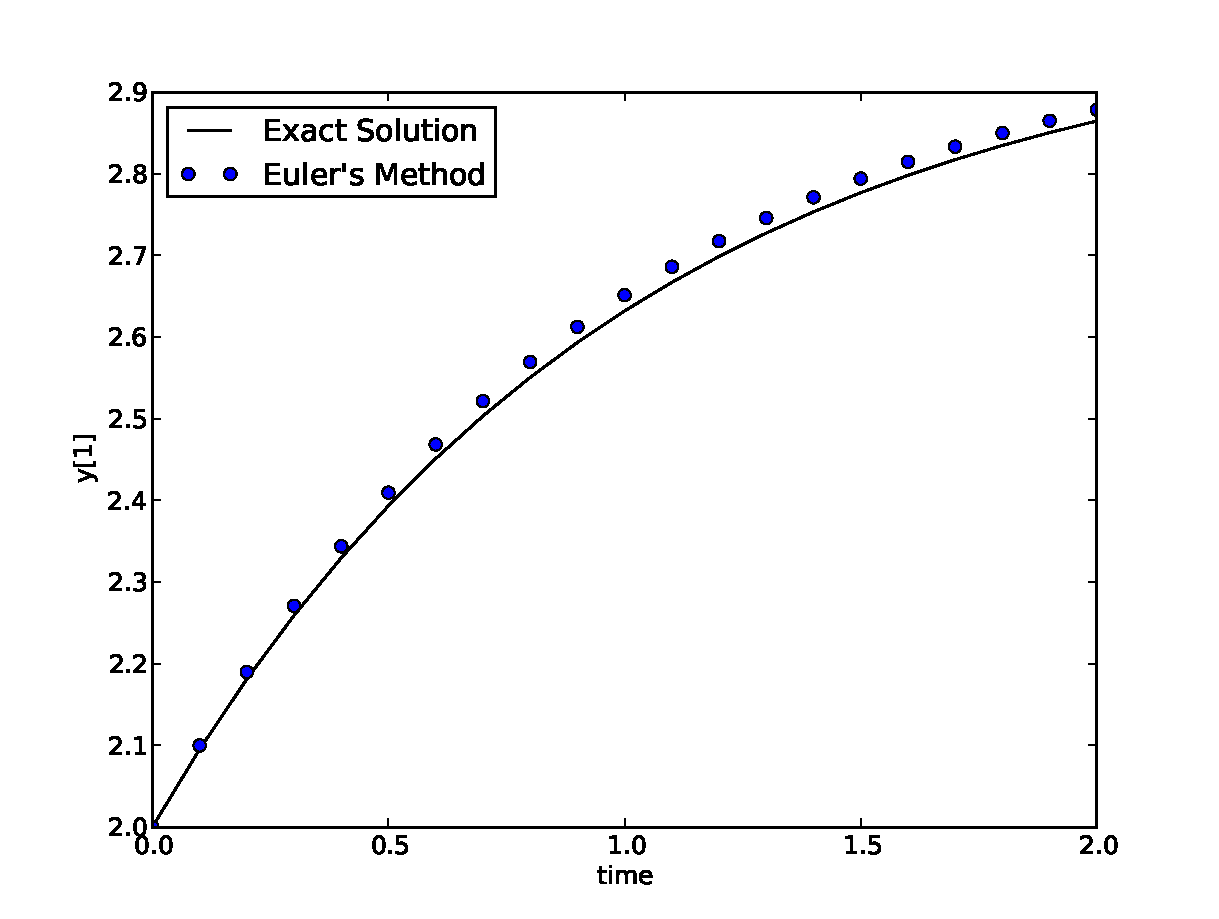
\includegraphics[width=3.25in,keepaspectratio=true]{./p4_2.pdf}
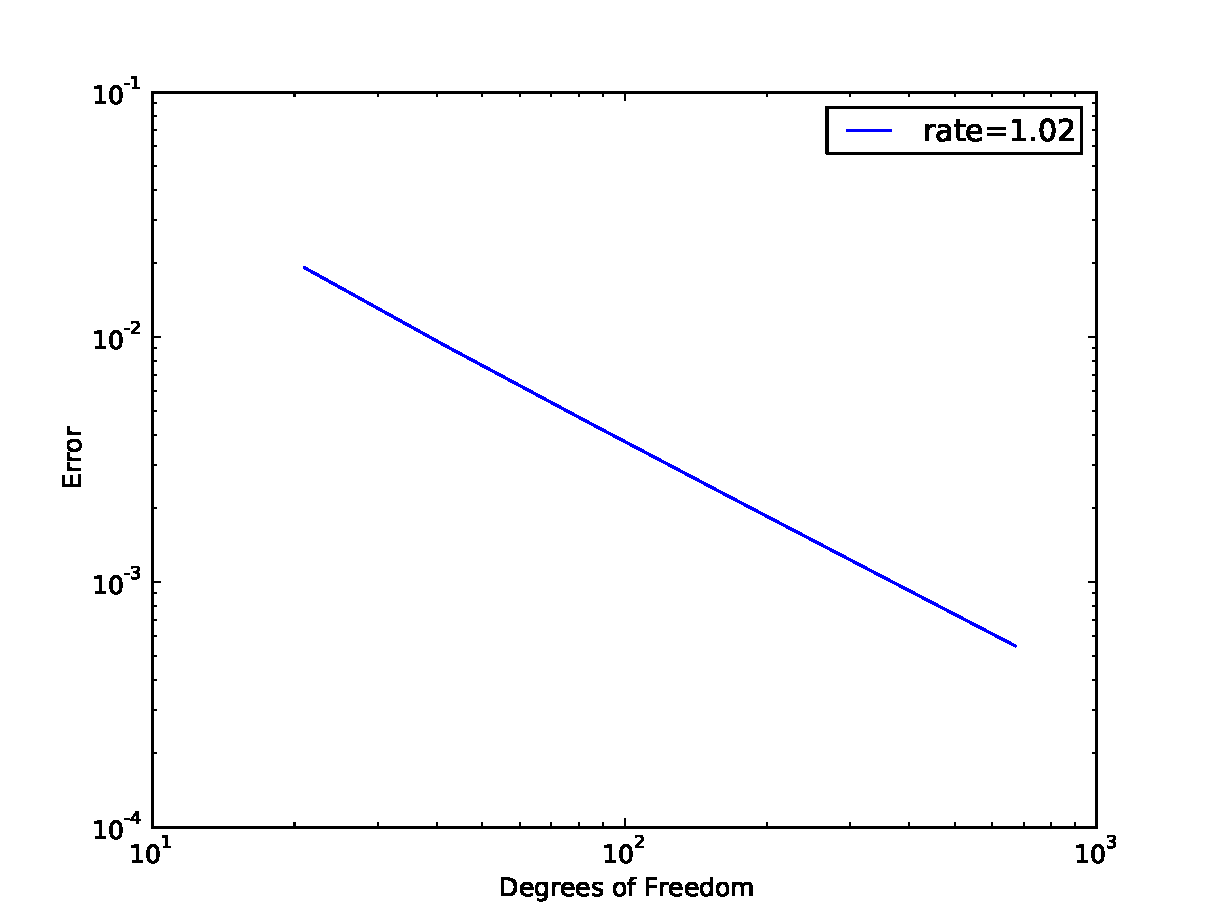
\includegraphics[width=4in,keepaspectratio=true]{./p4_3.pdf}
\caption{Problem 4}
\end{figure}

\subsection*{Test Problem 5}
\begin{align*}
\f(t,\y) &= -1/y)\\
\y(0) &= 1
\end{align*}
Exact Solution:
\[
\y(t)=\sqrt{1-2t}
\]
\begin{figure}[h!]
\centering
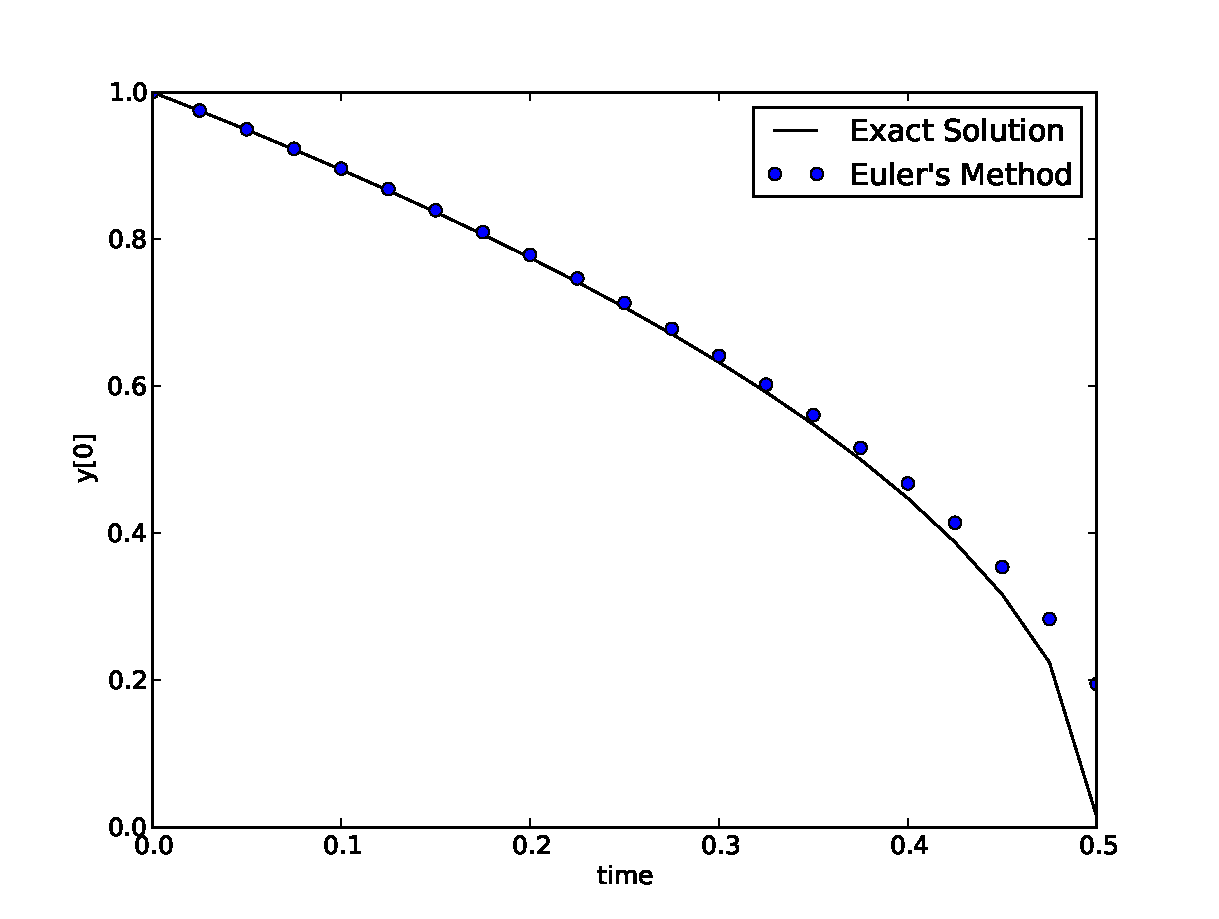
\includegraphics[width=3.25in,keepaspectratio=true]{./p5_1.pdf}
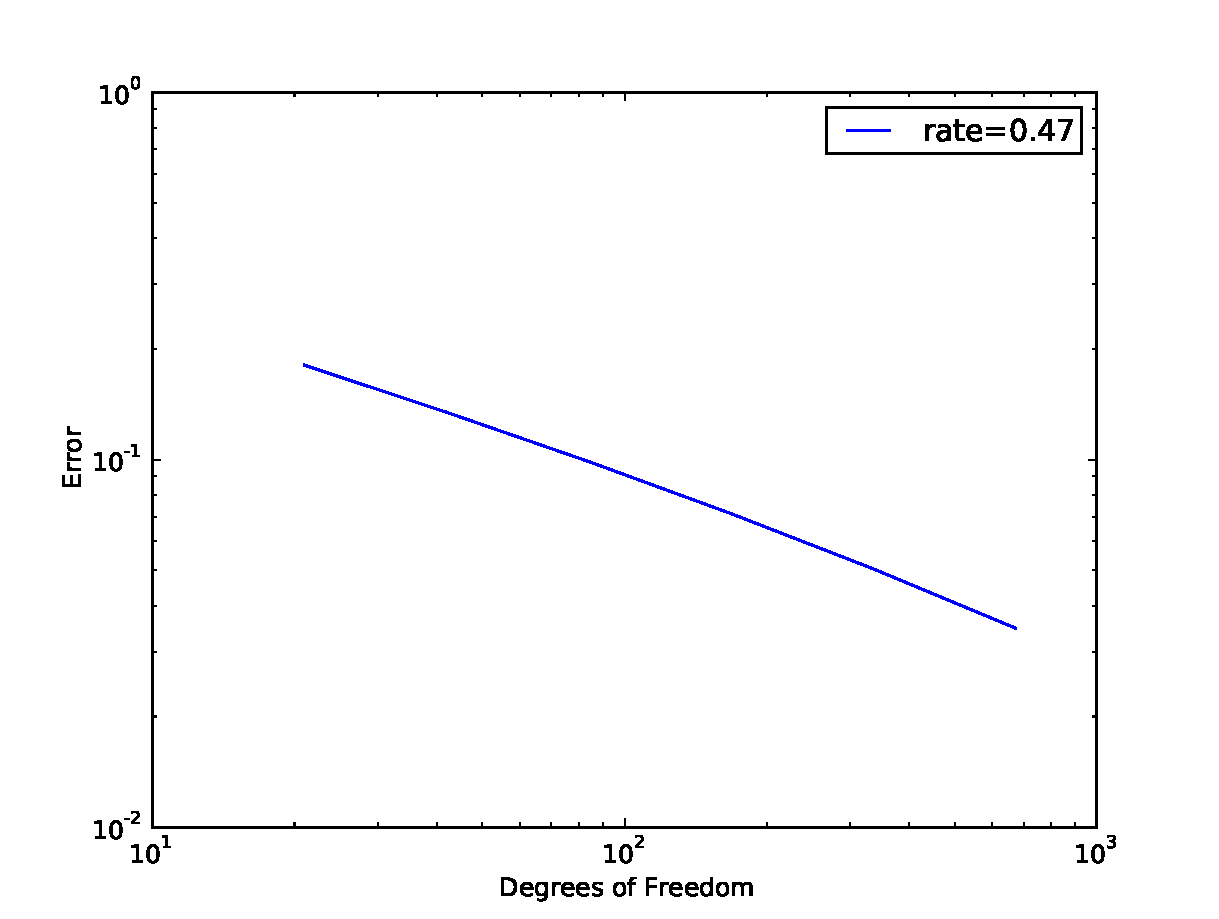
\includegraphics[width=3.25in,keepaspectratio=true]{./p5_2.pdf}
\caption{Problem 5}
\end{figure}

Problem 5 is not Lipshitz in $y$, therefore the convergence is not optimal.

\newpage 
\clearpage

\lstinputlisting[language=C++,title={Euler.cpp}]{Euler.cpp}
\lstinputlisting[language=Python,title={EulerPlot.py}]{EulerPlot.py}

\end{document}